\chapter{Future Work}\label{C:future}

\section{Weighting}
As mentioned during the preliminary evaluation chapter, the weighting is currently not achieving its purpose. The purpose was to remove the number of false-positives that are being identified however in the example shown it failed to do so. To achieve this, manual comparisons of the spectra before and after weighting will need to be examined. The reason is to try and determine the effect on the level of false-positives that method execution spectra has and may give insight whether it is worth pursuing the weighting feature further.

\section{Analysis Methods}
Different metrics will need to be implemented along with gathering more information from the paper trail. As noted in Section \ref{S:trace}, AspectJ allows us access to parameter values within a point cut. The idea that is proposed is to hold ranges of primitive values. For example, true and false would be held, and for number values, the values that would be held are negative, zero and positive. This gives us more information such as when an edge case is being tested with a negative value. To hold every value would be unnecessary, as the range suggested gives us enough information without adding too much to the potential scope of the test cases. Although it would be appropriate to hold object parameters, this is not viable except for string and null references. Since this would require every object to have a method where it gives enough details about that object. Although there is a toString() method, this is not always overridden or gives enough information.

Shown in Chapter \ref{C:evaluation} is a basic GUI, showing limited information. This GUI will have to be improved to show statistics of the test suite, this will not only help developers but also during the evaluation of the results. Since this project is to not say whether two tests are redundant, but to suggest potential redundant tests, it should be easy to explore these tests.

\section{Evaluation}
The method of evaluation is going to be how well the framework allows for redundant tests to be identified. The range of algorithms implemented will be executed and the results examined. To do this examination, manual inspection of the tests will have to be done in order to judge how well the framework is identifying potential redundant tests. Doing this manual inspection vs metric comparison will show the percentage of redundant vs false-positive test cases. During this manual inspection, liaison with Dr David Pearce will provide crucial feedback in determining the level of redundancy due to his experience. However, by using actively developed benchmarks, it allows for developers of these to potentially have a say on the level of redundancy as well. 

Some of the items that will be examined during this evaluation are: pipeline vs non-pipeline, weighting, spectra comparison and metric comparison.

\section{Final Report}
A final report will be written to give an in depth analysis on this research. This will include analysing and evaluating the results and coming to a conclusion of whether this framework has potential to be useful in an active development environment. 

\section{Requests for feedback}
How much information should the GUI show? Should the GUI show just enough information to help during the evaluation stage, or should more be provided in an effort to give it more use-ability?

\begin{figure}[h]
\centering
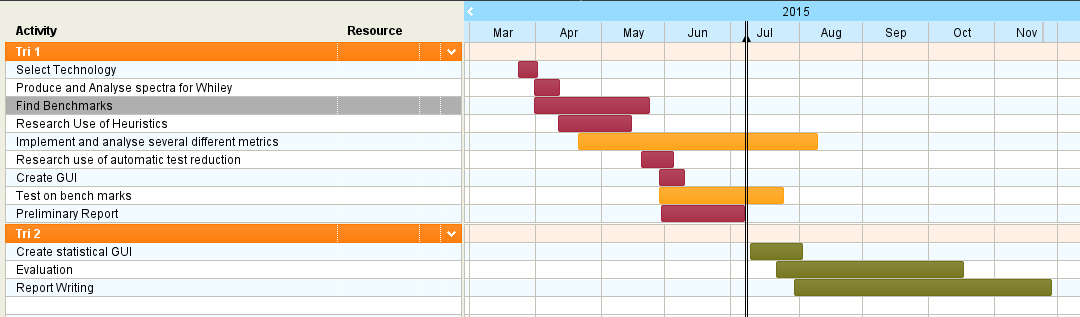
\includegraphics[width=17cm,height=7cm]{model28.png}
\caption{Gantt Chart}
\label{fig:gantt}
\end{figure}